\documentclass[11pt]{article}
\usepackage{icmlko}
\begin{document}

\title{어제의 규칙을 오늘 반증했다 --- 절단이 아니라 바닥 아래에서 축이 통하느냐다}
\author{월드모델 실험실}
\date{노트 385 · 2026년 8월 1일}
\maketitle

\begin{abstract}
노트 384가 규칙 하나를 세웠다: \emph{수집 편향이 도메인 점수를 부풀리는
것은 거른 축과 라벨이 같은 양일 때다.} 펀딩은 쪽 순서와 후원자 수가 같은
양이라 무너졌고($+0.3746 \to +0.0667$), 게임은 \texttt{topsellers}(총 판매)와
\texttt{y\_w30}(30일 창 리뷰)이 다른 양이라 안 무너졌다($p=0.155$)는
설명이었다.

\textbf{한 도메인 안에서 시험할 수 있는 규칙이라 시험했고, 틀렸다.}
게임의 라벨을 \texttt{y\_w30} 에서 \texttt{y\_raw}(총 리뷰)로만 바꾸면
거른 축과 라벨이 \emph{같은 양}이 된다 --- 나머지는 전부 같다. 사전 등록:
그러면 옛(위 0.36\%)과 균일의 간격이 \textbf{벌어져야} 한다.

\begin{center}
\begin{tabular}{lrrrr}
\hline
라벨 & 옛 $\rho$ & 균일 $\rho$ & 차 & $p$ \\
\hline
\texttt{y\_w30} (거른 축과 다름) & $+0.4931$ & $+0.3773$ & $+0.1158$ & 0.155 \\
\texttt{y\_raw} (거른 축과 \textbf{같음}) & $+0.3914$ & $+0.3701$ & $\mathbf{+0.0213}$ & 0.794 \\
\hline
\end{tabular}
\end{center}

\textbf{간격이 오히려 줄었다.} 예측과 반대다.

\textbf{그런데 기제의 절반은 맞았다.} 라벨을 바꾸자 균일 225행 중 옛 바닥
아래가 \textbf{0에서 184개(82\%)}로 늘었다 --- ``거른 축과 라벨이 같으면
위를 뜨는 것이 곧 라벨 아래를 자르는 것''은 정확했다. \textbf{틀린 것은
그 다음 고리다: 잘렸다고 점수가 부풀지는 않는다.}

그러면 무엇이 가르나. 잘려 나간 구간을 따로 채점하니 답이 나왔다:

\begin{center}
게임 바닥 아래 184행 $\mathbf{+0.2746}$ \quad 대 \quad
세계애니 99행 $+0.0223$(노트 376) \quad 대 \quad
펀딩 157행 $\mathbf{-0.0094}$(노트 379)
\end{center}

\textbf{고친 규칙: 위를 뜬 것 자체는 점수를 안 부풀린다. 부풀리는 것은
잘려 나간 구간에서 축이 안 통할 때다.} 게임은 바닥 아래에서도 축이
통하므로($+0.2746$) 위쪽 표본으로 잰 점수가 전체를 대표한다. 펀딩과
세계애니는 안 통하므로 위쪽 점수가 전체의 값이 아니다.

이 규칙은 노트 376이 이미 만들어 둔 절차로 곧장 잰다 --- 바닥 아래를
받아 따로 채점한다. \textbf{새 검사를 만들 필요가 없었고, 노트 384가
만든 검사(``거른 축과 라벨이 같은 양인가'')는 버린다.}
\end{abstract}

\section{왜 하루 만에 시험할 수 있었나}

노트 384의 규칙은 \emph{도메인 사이}를 견주는 설명이었다 --- 펀딩은 이렇고
게임은 저렇다. 그런 설명은 도메인마다 다른 것이 스무 가지라 확인이 어렵다.
그런데 이 규칙은 운 좋게 \textbf{한 도메인 안에서} 시험할 수 있었다.
게임에는 라벨이 둘 있다:

\begin{itemize}
\item \texttt{y\_raw} --- 총 리뷰 수. 수집이 \texttt{filter=topsellers} 로
줄 세운 것과 \emph{같은 양}이다.
\item \texttt{y\_w30} --- 출시 30일 창 리뷰(노트 210이 누적 라벨을 고치려고
바꾼 것). \emph{다른 양}이다.
\end{itemize}

같은 행 · 같은 축 · 같은 모형에서 라벨만 갈아 끼우면 규칙이 지목하는
변수 하나만 바뀐다. \textbf{그래서 사전 등록하고 돌렸다.}

\begin{figure}[t]
\centering
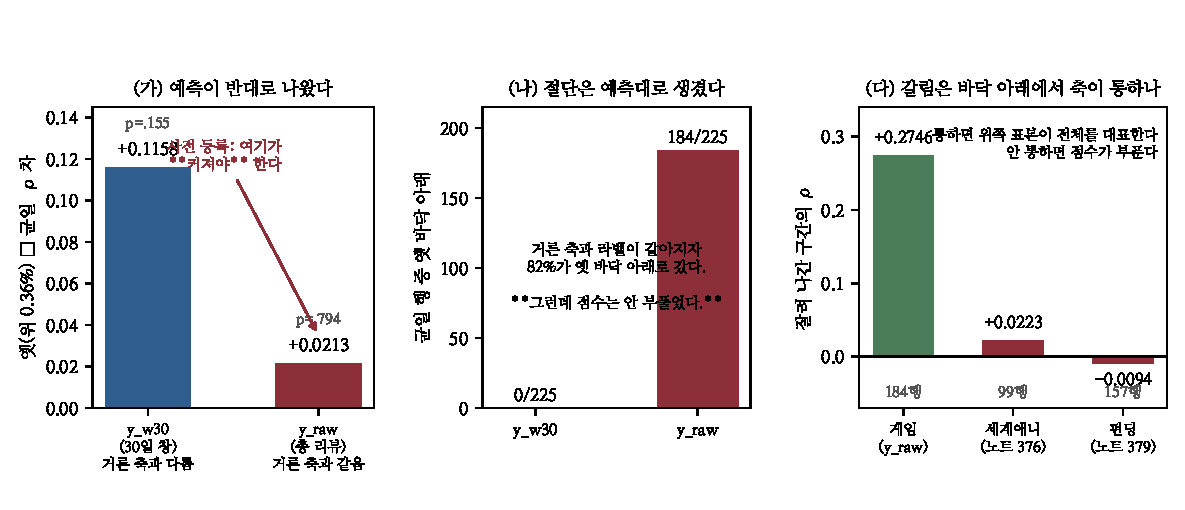
\includegraphics[width=\linewidth]{figs/fig385.pdf}
\caption{\textbf{(가)} 사전 등록은 \texttt{y\_raw} 에서 간격이 커진다는
것이었는데 $+0.1158 \to +0.0213$ 으로 줄었다. \textbf{(나)} 기제의 절반은
맞았다 --- 라벨을 바꾸자 균일 행의 82\%가 옛 바닥 아래로 갔다.
\textbf{(다)} 진짜 갈림은 잘려 나간 구간에서 축이 통하느냐다.}
\label{fig:main}
\end{figure}

\section{어디까지 맞았고 어디서 틀렸나}

규칙은 두 고리였다.

\textbf{고리 1 --- 거른 축과 라벨이 같으면 라벨 아래가 잘린다. 맞았다.}
\texttt{y\_w30} 에서는 균일 225행 중 옛 바닥($82$개 리뷰) 아래가 0개인데,
\texttt{y\_raw} 로 바꾸면 옛 바닥이 총 리뷰 82가 되고 균일 중앙이 11이라
\textbf{184개(82\%)}가 그 아래로 간다. 예측한 그대로다.

\textbf{고리 2 --- 잘리면 점수가 부푼다. 틀렸다.} 82\%가 잘려 나간 상태에서
옛 $+0.3914$ 대 균일 $+0.3701$ 로 사실상 같다($p=0.794$).

\textbf{두 고리를 하나로 묶어 쓴 것이 잘못이었다.} 절단은 \emph{표본이
모집단을 안 덮는다}는 사실이고, 점수 부풀림은 \emph{덮인 데서 잰 수가
안 덮인 데를 대표 못 한다}는 사실이다. 둘은 다른 말이고, 뒤엣것은 안
덮인 데를 실제로 재 봐야 안다.

\section{고친 규칙과 그 근거}

잘려 나간 구간만 따로 채점하면 세 도메인이 깨끗이 갈린다.

\begin{center}
\begin{tabular}{lrrl}
\hline
도메인 & 바닥 아래 행 & 그 구간 $\rho$ & 위쪽 점수가 부풀었나 \\
\hline
게임 (\texttt{y\_raw}) & 184 & $\mathbf{+0.2746}$ & 아니다 ($p=0.794$) \\
세계애니 (노트 376) & 99 & $+0.0223$ & 넓힐 수 없었다 \\
펀딩 (노트 379) & 157 & $\mathbf{-0.0094}$ & 그렇다 ($4.8$배) \\
\hline
\end{tabular}
\end{center}

\textbf{바닥 아래에서 축이 통하면 위쪽 표본으로 잰 점수가 전체를
대표한다.} 게임은 $+0.2746$ 으로 통하고, 그래서 위 0.36\%만 봤어도 점수가
안 부풀었다. 펀딩은 $-0.0094$, 세계애니는 $+0.0223$ 으로 안 통하고,
그래서 위쪽 점수가 전체의 값이 아니었다.

\textbf{검사는 이미 있다.} 노트 376이 세계애니에서 만든 절차 그대로다 ---
바닥 아래를 받아 유보에만 넣고 한 번의 적합 안에서 따로 채점한다. 노트
384가 만든 검사(``거른 축과 라벨이 같은 양인가'')는 \textbf{버린다} ---
필요조건에 가깝지만 충분조건이 전혀 아니고, 충분조건 노릇을 하라고 만든
검사였다.

\textbf{읽는 법도 바뀐다.} 노트 382가 만든 바닥 표(웹툰 19 · 게임 82 ·
만화 633 · 아이돌 772 · 도서 950 · 세계애니 19,533)는 \emph{어디를 재
봐야 하는지}의 목록이지 \emph{어디가 부풀었는지}의 목록이 아니다. 바닥이
제일 높은 세계애니는 넓혀도 소용이 없었고, 바닥이 낮은 게임은 애초에
문제가 없었다. \textbf{바닥의 높이는 답이 아니라 질문이다.}

\section{남은 것}

\begin{center}
\begin{tabular}{lll}
\hline
항목 & 왜 값이 큰가 & 어떻게 \\
\hline
만화 바닥 아래 & 무게 258 · 바닥 633 · 아직 안 쟀다 & 노트 376 절차 \\
아이돌 바닥 아래 & 바닥 772 에 구역 편향까지 & 무게 51 이라 뒤 \\
왜 어디선 통하고 어디선 안 통하나 & 고친 규칙의 다음 층 & 세 도메인 축 덮음 · 라벨 성질 비교 \\
도서 & 열거 경로를 못 찾았다 & 알라딘 다른 API 역설계 \\
\hline
\end{tabular}
\end{center}

\end{document}
